\section{Desarrollo Experimental 1}
Para esta primera actividad, aprenderemosa calibrar la punta de osciloscopio, para ello conectaremos la punta en la misma entrada del osciloscopio, asegurandonos de que la punta esté en x10 de atenuación, luego con un destornillador ajustaremos el trimer de calibración hasta que la señal que se muestra en el osciloscopio tenga la siguiente forma de onda.


\begin{figure}[H]
	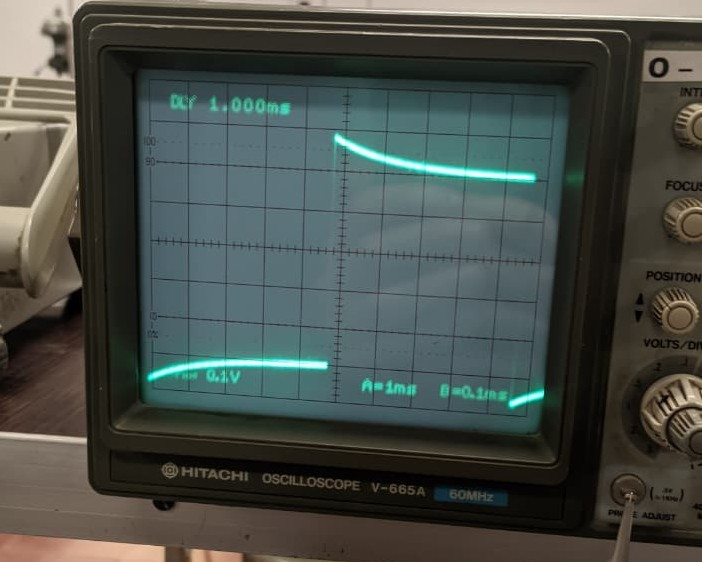
\includegraphics[width=0.4\textwidth]{images/calibraciona.jpeg}
	\caption{Señal de calibración del osciloscopio}
	\label{fig:calibracion}
\end{figure} 

Luego conectaremos la punta a la salida del generador de funciones, y ajustaremos el generador para que entregue una señal senoidal efectuando un barrido desde 100 Hz hasta 1 MHz, y obtendremos las siguientes amplitudes:

Ahora podremos armar un grafico con la relación entre la frecuencia y la amplitud.

A continuación volveremos a conectar la punta del osciloscopio al mismo osciloscopio, y ajustaremos el trimer de calibración para que la señal tenga la siguiente forma de onda.

\begin{figure}[H]
	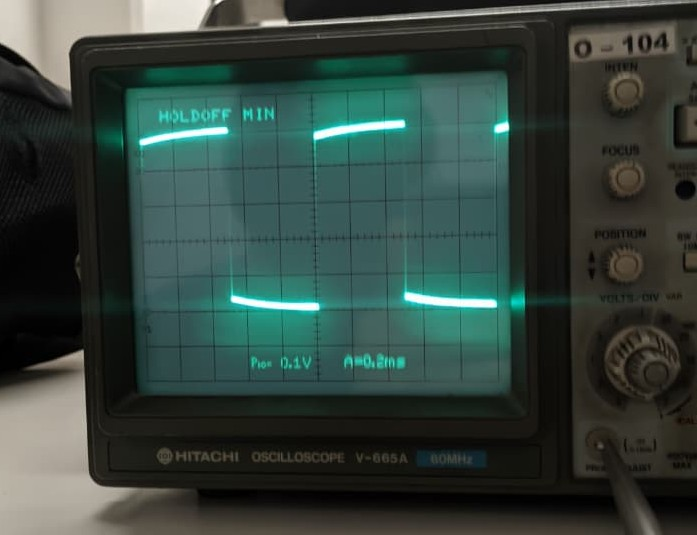
\includegraphics[width=0.4\textwidth]{images/calibracionb.jpeg}
	\caption{Señal de calibración del osciloscopio}
	\label{fig:calibracion}
\end{figure} 

Realizamos los mismos pasos y obtendremos las siguientes amplitudes:

Ahora podremos armar un grafico con la relación entre la frecuencia y la amplitud.

Para finalizar esta primera actividad, conectaremos la punta del osciloscopio nuevamente, pero ahora ajustaremos el trimer de calibración para que la señal tenga la siguiente forma de onda, la que sería la calibrada.

%\begin{figure}[H]
% 	\centering
%	\includegraphics[width=0.5\textwidth]{images/calibracionc.jpeg}
%	\caption{Señal de calibración del osciloscopio}
%	\label{fig:calibracion}
%\end{figure} 

Nuevamente tomamos datos de las amplitudes.

Y obtendremos el siguiente grafico con la relación entre la frecuencia y la amplitud.

Completando las frases tendremos que:

A.	El oscilograma \_\_\_ corresponde a ``caída de respuesta en frecuencias elevadas''.

B.	El oscilograma \_\_\_ corresponde a ``exceso de respuesta en frecuencias elevadas''.

C.	El oscilograma \_\_\_ corresponde a ``respuesta plana''.

\section{Desarrollo Experimental 2}

Para la actividad 2 encenderemos el generador de funciones y pondremos una onda cuadrada de aproximadamente 50Hz, con la amplitud de salida al máximo. Conectaremos la punta en x1 y ajustaremos los controles del osciloscopio para visualizar la señal y cambiaremos el acoplamiento de la entrada vertical de CC a CA y veremos la siguiente señal:

\begin{figure}[H]
	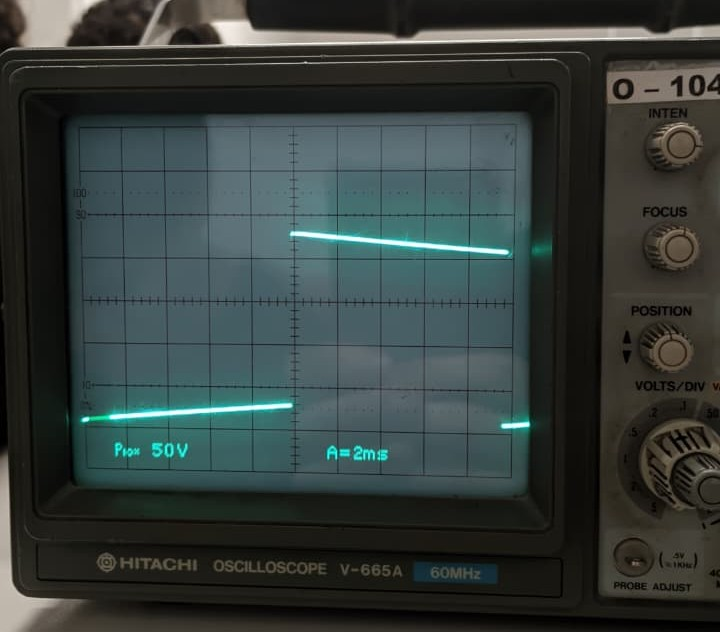
\includegraphics[width=0.4\textwidth]{images/parte2.jpeg}
	\caption{Señal en x1 con acoplamiento en CA}
	\label{fig:calibracion}
\end{figure} 

Ahora cambiaremos la punta a x10 y veremos lo siguiente:

\begin{figure}[H]
	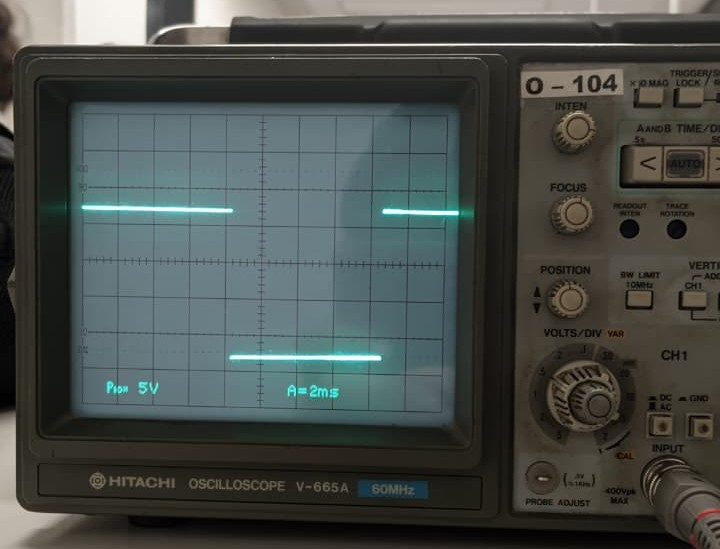
\includegraphics[width=0.4\textwidth]{images/parte2b.jpeg}
	\caption{Señal en x10 con acoplamiento en CA}
	\label{fig:calibracion}
\end{figure} 


\section{Desarrollo Experimental 3}

Para esta parte, dispondremos de una fuente sin regular, disponible en el pañol, para ello encenderemos la fuente y conectaremos como carga de la salida regulada un resistor de 39$\Omega$ de por lo menos 5W, y luego consiguramos el ocsiloscopio de la siguiente manera para efectuar mediciones de Vcc:

En primer lugar el modo de disparo en automático, un valor de sensibilidad acorde con el nivel de tensión que se espera medir, luego llevaremos el selector de acoplamiento a GND para colocar la línea de base en un lugar cómodo, y volveremos a CC.

Ahora conectamos la punta de pruebas del osciloscopio a la salida sin regular:

\begin{figure}[H]
	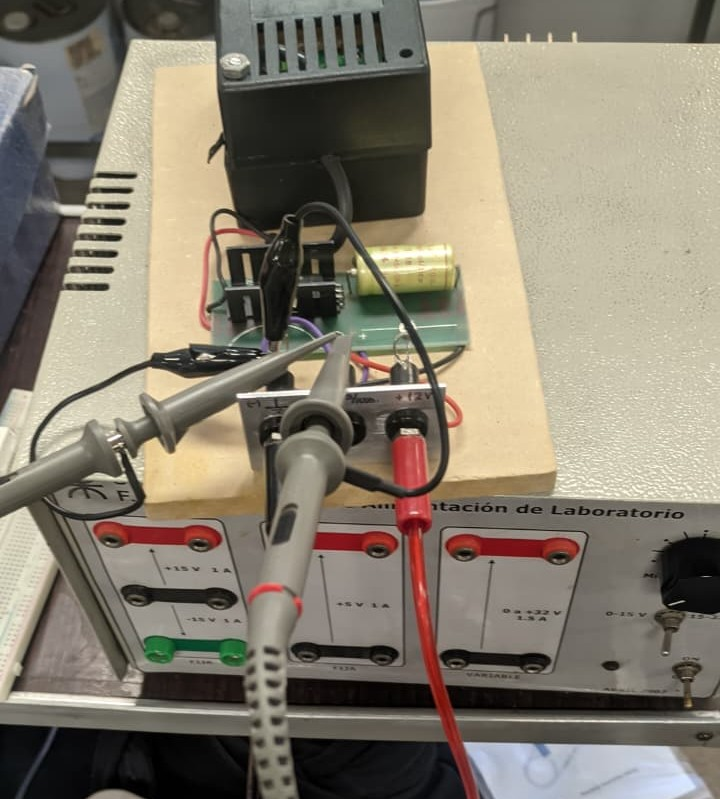
\includegraphics[width=0.4\textwidth]{images/parte3a.jpeg}
	\caption{Señal en x10 con acoplamiento en CA}
	\label{fig:calibracion}
\end{figure} 

Mediremos la amplitud de la señal, teniendo en cuenta que la punta esta en x10. Obtendremos los siguientes valores:

\begin{figure}[H]
	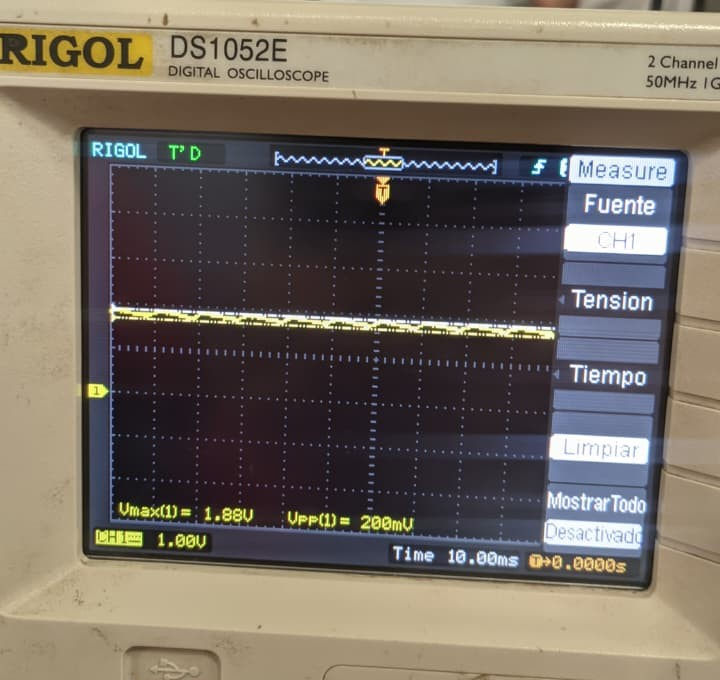
\includegraphics[width=0.4\textwidth]{images/parte3b.jpeg}
	\caption{Señal en x10 con acoplamiento en CA}
	\label{fig:calibracion}
\end{figure} 


$$V_{cc}=1.88V$$

Ahora intentaremos visualizar el ripple, para ello cambiaremos el acoplamiento a CA y usaremos el disparo ''Interno'' de la base de tiempo y mediremos:

\begin{figure}[H]
	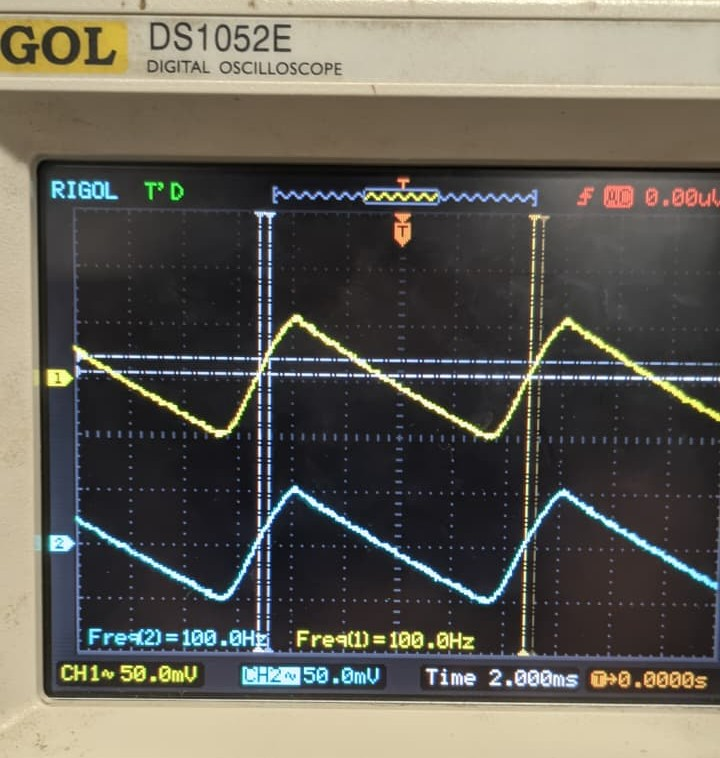
\includegraphics[width=0.4\textwidth]{images/parte3c.jpeg}
	\caption{Señal en x10 con acoplamiento en CA}
	\label{fig:calibracion}
\end{figure} 

$$V_{ripple}=$$

Como se dificulta ahustar el disparo debido a la forma de onda con mucho ruido, usaremos el disparo por ''Línea'' y ahora podremos determinar los siguientes datos:

$$T=$$
$$V_{pp}=$$

Y completamos las siguientes frases:

A. La frecuencia del ripple es \_\_\_.

B. El porcentaje de ripple respecto del valor Vcc es del \_\_\_.

\section{Desarrollo Experimental 4}

En esta parte usaremos el disparo interno del osciloscopio, el trigger. Para ello pondremos el generador de funciones con los siguientes datos:


\begin{table}[H]
\resizebox{\columnwidth}{!}{%
\begin{tabular}{|c|c|c|}
\hline
\textbf{Frecuencia} & \textbf{Función} & \textbf{Amplitud} \\ \hline
500 Hz              & Senoidal         & 5Vpp              \\ \hline
\end{tabular}%
}
\end{table}

Ahora conectamos el osciloscopio al generador y coon el acoplamiento en ''Interno'', seleccionamos la ''Pendiente'' o ''Slope'' en Positivo, y reulamos el nivel de disparo.

\begin{figure}[H]
	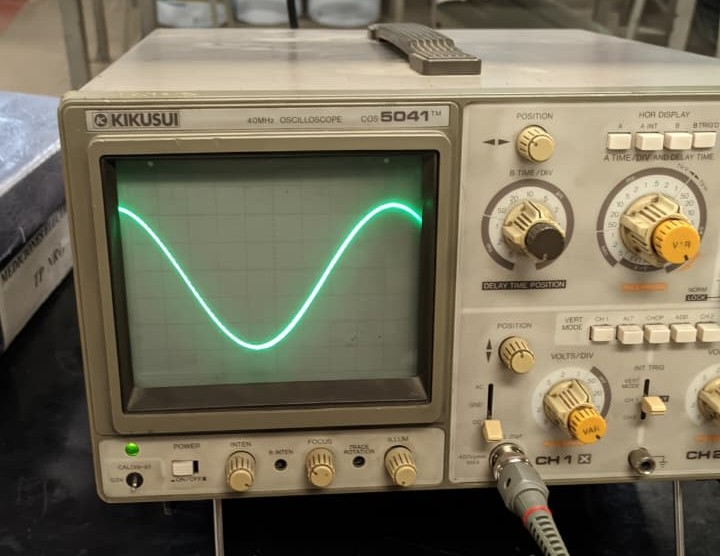
\includegraphics[width=0.4\textwidth]{images/parte4a.jpeg}
	\caption{Señal en x10 con acoplamiento en CA}
	\label{fig:calibracion}
\end{figure} 

Invertimos el control de ''Pendiente'' y obtendremos lo siguiente

\begin{figure}[H]
	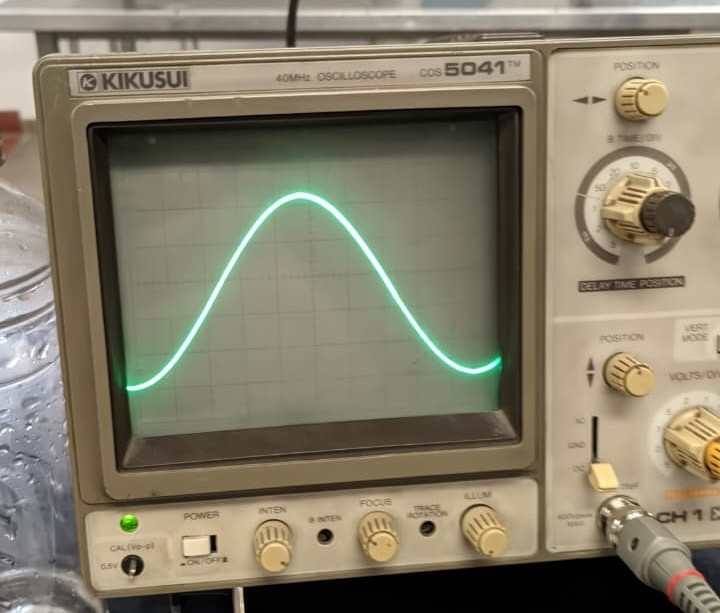
\includegraphics[width=0.4\textwidth]{images/parte4b.jpeg}
	\caption{Señal en x10 con acoplamiento en CA}
	\label{fig:calibracion}
\end{figure} 

Luego pondremos el generador con una onda cuadrada, de amplitud 300mVpp y reajustamos el nivel de disparo 

\begin{figure}[H]
	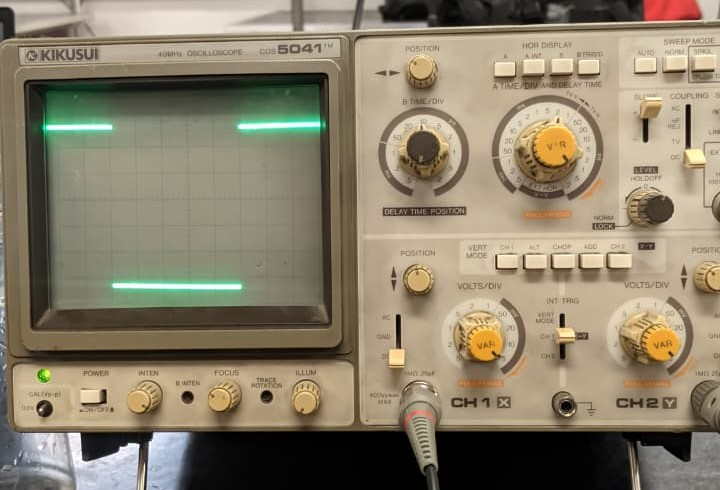
\includegraphics[width=0.4\textwidth]{images/parte4c.jpeg}
	\caption{Señal en x10 con acoplamiento en CA}
	\label{fig:calibracion}
\end{figure} 

Reducimos presentación con el vernier de ganancias del amplificado, hasta obtener lo siguiente:

\begin{figure}[H]
	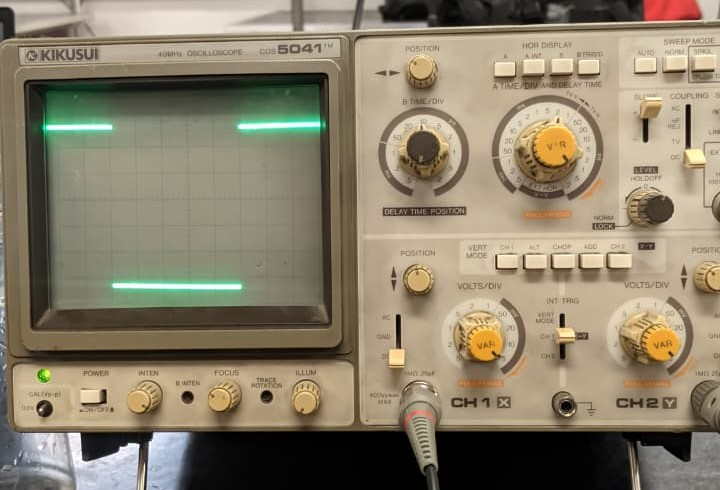
\includegraphics[width=0.4\textwidth]{images/parte4c.jpeg}
	\caption{Señal en x10 con acoplamiento en CA}
	\label{fig:calibracion}
\end{figure} 

Cuadro de controles:

\begin{table}[H]
\resizebox{\columnwidth}{!}{%
\begin{tabular}{|l|l|l|l|l|}
\hline
V/div (Y1)                & V/div (Y2)               & T/div & Aten Y1                  & Aten Y2                  \\ \hline
\multicolumn{1}{|c|}{5mV} & \multicolumn{1}{c|}{5mV} & 0.2ms & \multicolumn{1}{c|}{x10} & \multicolumn{1}{c|}{x10} \\ \hline
\end{tabular}%
}
\end{table}

Completamos la siguiente frase:

El nivel mínimo de señal que activa el circuito del trigger es de 1V/divisiones de la pantalla.